\section{Результаты}

В результате работы программы создаются родительский и два дочерних процесса. PID каждого процесса выводится в консоль.

Пример работы программы:

\begin{alltt}
parent pid: 1761
child1 pid: 1762
child2 pid: 1763
Operating Systems, Semester 3, Lab 2        
operating_systems,_semester_3,_lab_2
\end{alltt}

Различные значения PID подтверждают создание родительского и двух дочерних процессов. Итоговая строка подтверждает корректную последовательную обработку данных: child1 переводит символы в нижний регистр, а child2 заменяет пробельные символы на \texttt{\_}.

На рисунке~\ref{fig:program-run} представлен результат запуска программы.

\begin{figure}[ht]
  \centering
  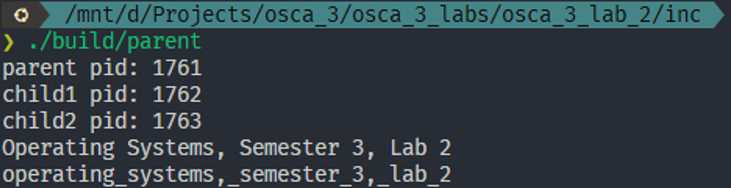
\includegraphics[width=0.7\textwidth]{program_run.png}
  \caption{Работа программы}
  \label{fig:program-run}
\end{figure}
